% !TeX spellcheck = en_US

\chapter{Image Segmentation with Convolutional Neural Networks (CNN)}
\section{Introduction}
With the increasing computational power that comes with recent graphic cards, increasingly complex neural networks can be used to achieve more challenging tasks than before. Such tasks can be object detection, where the goal is to determine whether an object of a specified class (for example 'car') is visible on a image. 

\begin{figure}[H]
    \centering
	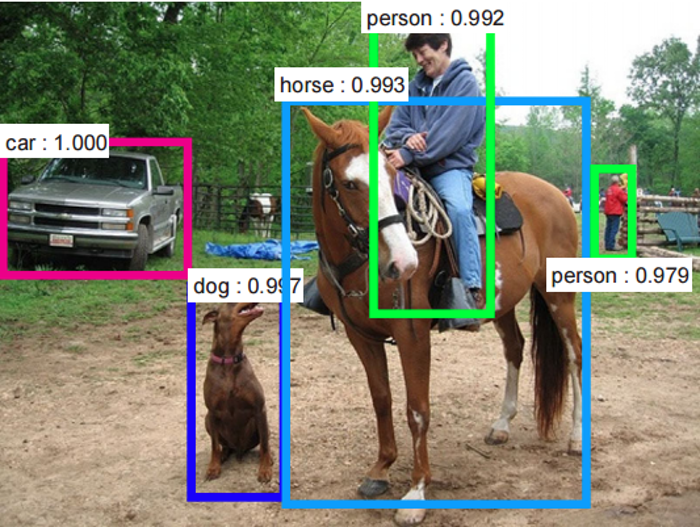
\includegraphics[width=0.6\linewidth]{chapters/neural_networks/images/object_detection.png}
	\caption{An example of object detection, showing the detected classes and the confidence of each prediction.\\ Source: https://dius.com.au/2016/12/06/the-cleverness-of-deep-learning/ (27.05.2018)}
	\label{fig:neural_networks:object_detection}
\end{figure}

In contrast to object detection, the target of image segmentation is not only to state whether an object could be found, but to label each pixel of an image with a class. The Different types of image segmentation can be seen in \autoref{fig:neural_networks:image_segmentation}.

\begin{figure}[H]
    \centering
	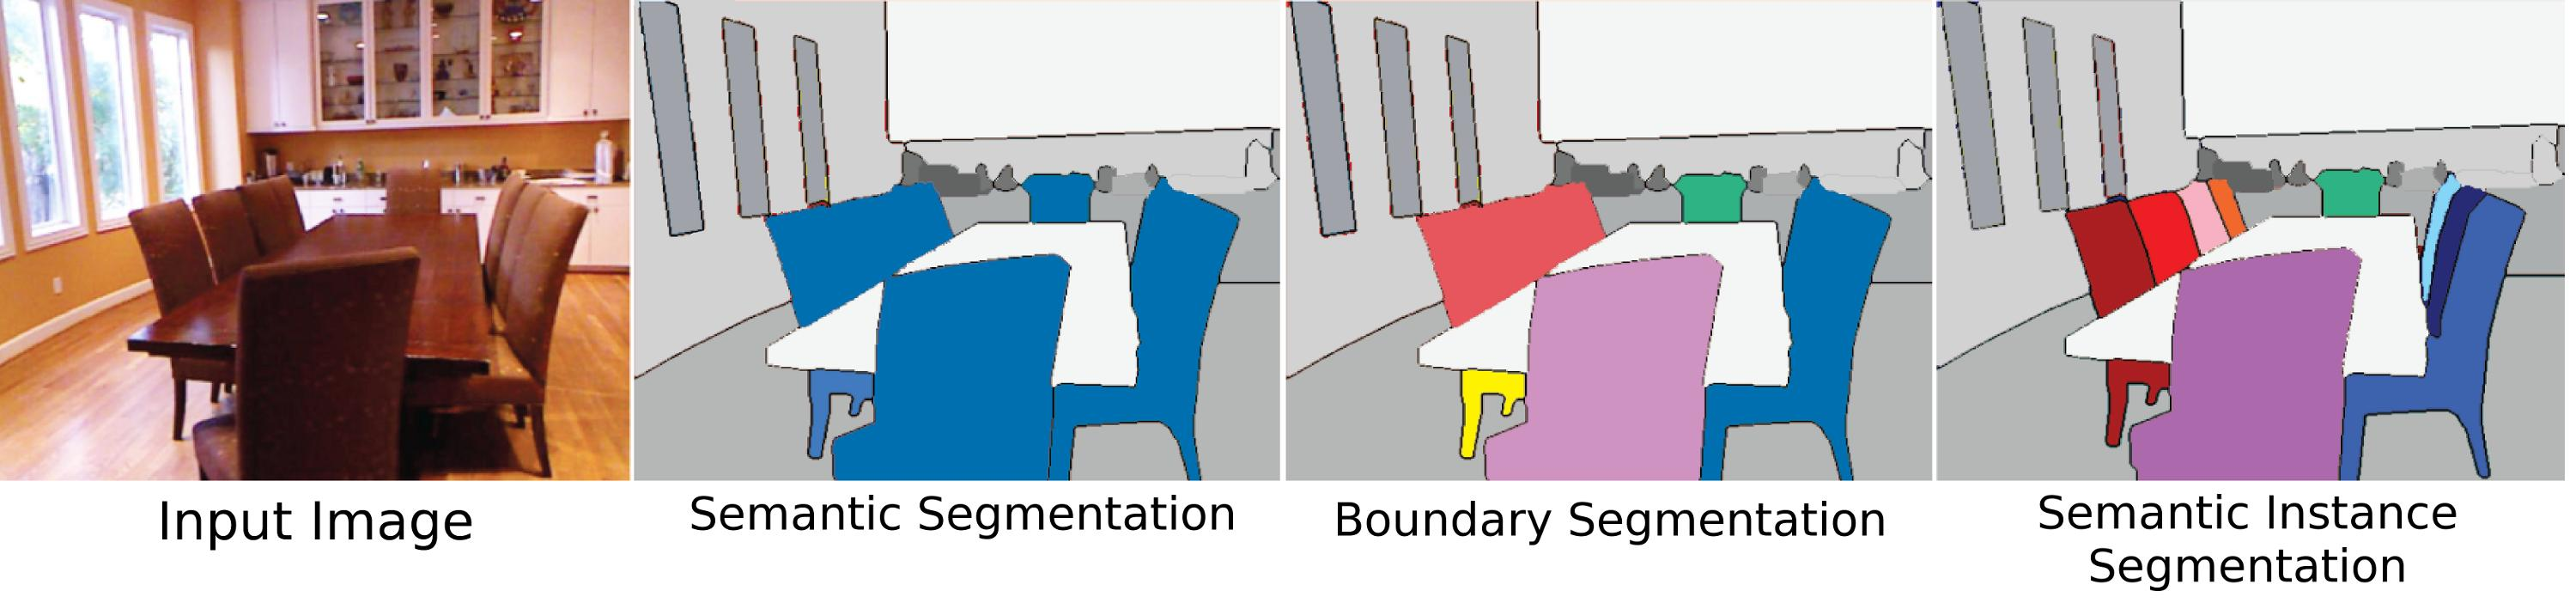
\includegraphics[width=0.8\linewidth]{chapters/neural_networks/images/segmentation.jpg}
	\caption{Different types of image segmentation.\\ Source: https://i.stack.imgur.com/mPFUo.jpg (27.05.2018)}
	\label{fig:neural_networks:image_segmentation}
\end{figure}

\section{Convolutional Layer}
A convolutional layer is one of the most important and basic building blocks of a neural network. It has a number of filters, each of which is small, compared to the input volume (the image), for example 5x5x3 pixels (a 5x5 filter with 3 channels, because standard images have 3 color channels). During the forward pass of the network, the filters are being moved over the input image and at each position of the filters on the image, a convolution is being computed, which is an element wise matrix multiplication and a sum over the resulting matrix. The result of this operation is an activation map, which is also the output of the convolutional layer.

Obviously, the size of a filter can be configured, as well as the step size, the stride, and the amount of zero padding around the input image.

\begin{figure}[H]
    \centering
	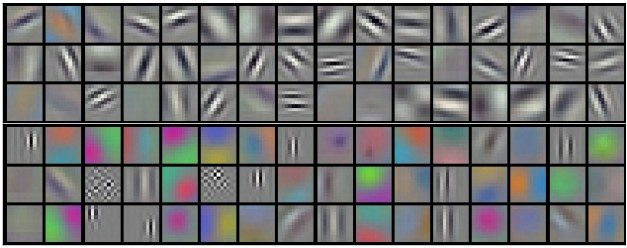
\includegraphics[width=0.6\linewidth]{chapters/neural_networks/images/example_filters.jpeg}
	\caption{Example filters learned by \cite{Krizhevsky.2012}.\\ Source: http://cs231n.github.io/assets/cnn/weights.jpeg (27.05.2018)}
	\label{fig:neural_networks:example_filters}
\end{figure}

\section{Pooling Layer}
Pooling is a technique which allows to reduce the size of an image by extracting a single value from a region of values. The extracted value depends on the pooling type that is used. Max pooling for example extracts the highest value from the region, whereas min pooling extracts the lowest value.

\begin{figure}[H]
    \centering
	\begin{subfigure}{0.4\textwidth}
    	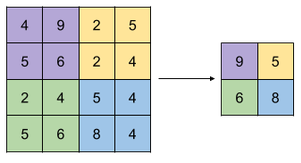
\includegraphics[width=0.9\linewidth]{chapters/neural_networks/images/max_pooling.png}		    \caption{Max Pooling}
    	\label{fig:challenges:max_pooling}
	\end{subfigure}~
	\begin{subfigure}{0.4\textwidth}
    	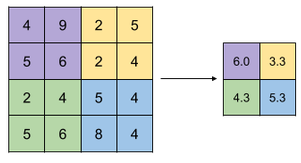
\includegraphics[width=0.9\linewidth]{chapters/neural_networks/images/avg_pooling.png}       	\caption{Average Pooling}
    	\label{fig:challenges:avg_pooling}
	\end{subfigure}
	\caption{Max and average pooling\\Source: https://idoml.com, 02.06.18}
	\label{fig:challenges:pooling}
\end{figure}

\subsection{Unpooling}
tbd

\section{Fully Connected Layer}
\section{Mask R-CNN}

